% =====================================================================
% CAPÍTULO 8: VALIDACIÓN Y PRUEBAS DEL SISTEMA
% Versión académica revisada con criterios de evidencia técnica
% =====================================================================

\chapter{Validación y Pruebas del Sistema}
\label{ch:validacion-pruebas}

% --- Ajustes editoriales locales del capítulo: sangría, espaciado y control de desbordamientos ---
\setlength{\parindent}{0pt}
\setlength{\parskip}{6pt}
\sloppy
\emergencystretch=2em
\raggedbottom
% Colores institucionales exigidos para diagramas y resaltados
\providecolor{institucionalRed}{HTML}{AD3333}
\providecolor{institucionalBlue}{HTML}{003366}
\providecolor{institucionalGrey}{HTML}{DADADA}

\section{Introducción a la validación}
\label{sec:introduccion-validacion}

La validación es el proceso metodológico utilizado para comprobar que el artefacto de software cumple los requisitos funcionales, técnicos y de seguridad definidos para el flujo operativo de CERMONT S.A.S. Para dotar al proyecto de rigor técnico verificable, la validación se organizó en dos niveles: primero, una batería de pruebas automatizadas orientada a verificar la integridad transaccional, la seguridad y la consistencia lógica del código; segundo, una matriz de aceptación funcional por rol, diseñada para contrastar el comportamiento del sistema frente a las necesidades de los usuarios de la organización.

\section{Arquitectura del entorno de pruebas automatizadas}
\label{sec:arquitectura-pruebas}

Para la ejecución y mantenimiento de la suite de pruebas del monorepo, se implementó un entorno de pruebas basado en \textbf{Vitest}, herramienta compatible con TypeScript y con el ecosistema Vite. La suite de pruebas interactúa directamente con los endpoints HTTP expuestos por el backend en Express utilizando la librería \textbf{Supertest}.

\begin{tikzpicture}[
  node distance=1cm,
  every node/.style={font=\scriptsize},
  box/.style={draw=institucionalBlue, rounded corners=3pt, fill=institucionalGrey!35, align=center, minimum width=3.0cm, minimum height=0.78cm, line width=0.75pt},
  result/.style={draw=institucionalRed, rounded corners=3pt, fill=institucionalRed!8, align=center, minimum width=3.0cm, minimum height=0.78cm, line width=0.85pt},
  arrow/.style={-{Latex[length=2mm]}, draw=institucionalBlue, line width=0.8pt},
  arrowred/.style={-{Latex[length=2mm]}, draw=institucionalRed, line width=0.8pt}
]
\node[box] (utilidad) {Utilidad percibida};
\node[box, right=of utilidad] (facilidad) {Facilidad de uso};
\node[result, right=of facilidad] (intencion) {Aceptación del sistema};
\node[box, below=of facilidad] (contexto) {Condiciones de campo\\y soporte documental};
\draw[arrow] (utilidad)--(facilidad);
\draw[arrowred] (facilidad)--(intencion);
\draw[arrow] (contexto)--(facilidad);
\draw[arrow] (contexto)--(utilidad);
\end{tikzpicture}


El entorno mantiene aislamiento frente a los datos de producción aplicando los siguientes patrones técnicos en el archivo de inicialización global \texttt{setup.ts}:
\begin{itemize}
    \item \textbf{Base de datos en memoria (Sandbox Mongoose)}: En lugar de conectarse a la instancia principal de MongoDB, el entorno de pruebas levanta y destruye dinámicamente un esquema temporal apuntando a la URI aislada \texttt{mongodb://127.0.0.1:27017/cermont\_test}. Esto asegura que las operaciones de creación, actualización y borrado de las pruebas no contaminen ni alteren los registros reales de la compañía.
    \item \textbf{Mocks Criptográficos}: Los procesos costosos de hashing de contraseñas de \textbf{Bcryptjs} se configuran temporalmente con un factor de ronda mínimo (\texttt{saltRounds = 1}) durante las pruebas, acelerando la velocidad de respuesta sin comprometer la lógica de validación de credenciales.
\end{itemize}

\section{Resultados cuantitativos y desglose de la suite de pruebas}
\label{sec:resultados-pruebas}

La ejecución automatizada debe conservarse en un reporte técnico anexo con salida de consola, fecha, entorno y versión del código evaluado. Esta evidencia valida el comportamiento técnico del artefacto, pero no sustituye la medición operativa en producción con usuarios reales. Si dicho reporte no se adjunta, el resultado queda pendiente por anexar evidencia.

A continuación se detalla la distribución y alcance temático de los bloques de pruebas reportados. La evidencia de consola, fecha, commit y entorno debe conservarse en el anexo de validación técnica para que la afirmación sea verificable por el jurado:

\subsection{Suite de Autenticación, Sesión y Seguridad (JWT HttpOnly)}
\begin{itemize}
    \item \textbf{Alcance}: Verificación del ciclo de vida del token de sesión. Se prueba la generación del JWT directo, su inyección automática en cookies de tipo HttpOnly con banderas restrictivas (\texttt{Secure; SameSite=Strict}), la expiración controlada y el proceso de refresco del token mediante el \texttt{refreshToken} transaccional.
    \item \textbf{Resultado}: Debe verificarse con la corrida documentada en anexos. Si no se adjunta salida de consola, queda pendiente por anexar evidencia.
\end{itemize}

\subsection{Suite de Control de Acceso Basado en Roles (RBAC Guards)}
\begin{itemize}
    \item \textbf{Alcance}: Validación del middleware de autorización. Se introducen payloads de prueba emulando los diferentes perfiles del sistema (Gerente, Residente, Técnico, HES, Supervisor, Administrativo, Cliente) y se verifica que el backend responda con un código HTTP 403 Forbidden ante cualquier intento de escalado de privilegios o ejecución de acciones prohibidas (ej. un técnico intentando borrar de forma lógica una orden de trabajo).
    \item \textbf{Resultado}: Debe verificarse con la corrida documentada en anexos. El bloqueo de accesos no autorizados solo debe afirmarse para los casos efectivamente evaluados.
\end{itemize}

\subsection{Suite de Esquemas Dinámicos y Custom Fields (Zod 4.x)}
\begin{itemize}
    \item \textbf{Alcance}: Pruebas de resiliencia y flexibilidad de esquemas. Se valida que la carga de formularios dinámicos y la adición de campos personalizados a las órdenes de trabajo respeten estrictamente la especificación del contrato de datos centralizado, rechazando de forma segura entradas maliciosas o mal formateadas.
    \item \textbf{Resultado}: Debe verificarse con la corrida documentada en anexos. Los rechazos de payloads inválidos deben mostrarse con casos de prueba o salida de consola.
\end{itemize}

\subsection{Suite de Reglas de Negocio de Órdenes de Trabajo}
\begin{itemize}
    \item \textbf{Alcance}: Verificación de la máquina de estados secuencial de la OT. Se valida que una orden no pueda saltar etapas de forma incorrecta (ej. pasar de Fase de Planeación a Fase de Acta firmada sin registrar el checklist HES ni adjuntar evidencias fotográficas), asegurando el cumplimiento estricto del flujo operativo.
    \item \textbf{Resultado}: Debe verificarse con la corrida documentada en anexos. Las transiciones inválidas deben reportarse únicamente para los casos de prueba ejecutados.
\end{itemize}

\subsection{Suite de Proyección de Casos de Servicio (ServiceCase Projection)}
\begin{itemize}
    \item \textbf{Alcance}: Pruebas de integración sobre el motor de agregación de datos de MongoDB. Se inyectan de forma simulada registros dispersos en múltiples colecciones de la base de datos (una solicitud de visita, una cotización aprobada, dos evidencias y una orden finalizada) y se invoca al servicio de proyección \texttt{ServiceCase}. Se valida que el motor retorne un consolidado financiero exacto del proyecto, identifique de forma automática el cuello de botella actual (bloqueadores en actas o SES) y calcule el siguiente paso transaccional de manera correcta.
    \item \textbf{Resultado}: Debe verificarse con la corrida documentada en anexos. La consistencia de cálculos agregados debe quedar respaldada por casos concretos.
\end{itemize}

\subsection{Suite de Generación Documental y pdf-lib}
\begin{itemize}
    \item \textbf{Alcance}: Pruebas funcionales de compilación binaria de documentos. Se evalúa el servicio de creación de informes técnicos y actas de entrega, validando que el módulo compile un búfer binario en PDF válido, con marcas de agua, firmas incrustadas y tablas dinámicas de costos sin corromper el archivo resultante.
    \item \textbf{Resultado}: Debe verificarse con la corrida documentada en anexos. La generación de archivos PDF válidos debe conservarse como evidencia técnica.
\end{itemize}

\subsection{Suite de Evidencias Foto-Geolocalizadas}
\begin{itemize}
    \item \textbf{Alcance}: Verificación de las restricciones de archivos multimedia. Se prueban cargas de imágenes de alta resolución simuladas, verificando la extracción de coordenadas GPS del metadato EXIF, validación del tamaño de archivo permitido y rechazo automático de extensiones potencialmente maliciosas.
    \item \textbf{Resultado}: Debe verificarse con la corrida documentada en anexos. La asociación de metadatos con la orden correspondiente queda pendiente por anexar evidencia si no se incluye el reporte.
\end{itemize}

\section{Matriz consolidada de pruebas del monorepo}
\label{sec:matriz-pruebas-consolidada}

La validación cuantitativa del sistema se sintetiza en la Tabla \ref{tab:matriz-pruebas}, que refleja el estado de cumplimiento verificado por la suite de pruebas del monorepo.

\begin{table}[!htbp]
\centering
\caption{Matriz final de validación y estado de cumplimiento técnico. Fuente: Elaboración propia.}
\label{tab:matriz-pruebas}

\small
\def\TestRow#1#2#3#4{\parbox[t]{2.4cm}{\raggedright #1} & \parbox[t]{4.7cm}{\raggedright #2} & \parbox[t]{4.7cm}{\raggedright #3} & \parbox[t]{2.4cm}{\raggedright #4}\\\hline}
\begin{adjustbox}{max width=\textwidth}
\begin{tabular}{|l|l|l|l|}
\hline\ClassicTableHeader
\textbf{Nivel de Prueba} & \textbf{Objetivo Tecnológico} & \textbf{Resultado Esperado} & \textbf{Estado} \\
\hline
\TestRow{Unitaria}{Validar reglas de negocio puras, hooks de Zustand y esquemas Zod en \texttt{shared-types}.}{Comportamiento lógico correcto y libre de efectos colaterales.}{\textbf{Verificado según reporte anexo}}
\TestRow{Integración}{Evaluar la comunicación asíncrona entre Express, Mongoose y MongoDB en memoria.}{Persistencia transaccional de datos y consistencia referencial.}{\textbf{Verificado según reporte anexo}}
\TestRow{Extremo a Extremo (E2E)}{Simular peticiones HTTP completas (\texttt{Supertest}) de login, creación de OT, checklist y cierre.}{Flujo secuencial continuo y manejo centralizado de errores.}{\textbf{Verificado según reporte anexo}}
\TestRow{Aceptación cualitativa}{Evaluar la interfaz adaptativa y la operación offline con usuarios por rol.}{Experiencia de usuario comprensible y flujo funcional sin bloqueos críticos.}{\textbf{Matriz propuesta / requiere acta de aceptación}}
\hline
\end{tabular}
\end{adjustbox}
\end{table}

\section{Validación cualitativa y de usabilidad por roles}
\label{sec:validacion-usuario-v}

Para complementar la verificación cuantitativa, se diseñó un marco de aceptación cualitativa con el fin de auditar la respuesta del sistema frente a los operarios finales de CERMONT S.A.S. La Tabla \ref{tab:aceptacion-roles} expone las pruebas cualitativas propuestas para validación por rol. Cuando existan actas o formatos firmados por usuarios, deberán anexarse como evidencia de aceptación.

\begin{table}[!htbp]
\centering
\caption{Matriz de aceptación cualitativa por perfil de usuario. Fuente: Elaboración propia.}
\label{tab:aceptacion-roles}
\small
\def\AcepRow#1#2#3#4{\parbox[t]{3.0cm}{\raggedright #1} & \parbox[t]{5.1cm}{\raggedright #2} & \parbox[t]{4.2cm}{\raggedright #3} & \parbox[t]{2.1cm}{\raggedright #4}\\\hline}
\begin{adjustbox}{max width=\textwidth}
\begin{tabular}{|l|l|l|l|}
\hline\ClassicTableHeader
\textbf{Rol del Operario} & \textbf{Acción del Sistema Evaluada} & \textbf{Criterio de Aceptación} & \textbf{Resultado} \\
\hline
\AcepRow{Técnico de Campo (TEC)}{Captura offline de checklists y evidencias fotográficas.}{Operación offline comprensible y sincronización posterior cuando aplique.}{Escenario propuesto / requiere acta}
\AcepRow{Residente de Obra (RES)}{Asignación de recursos y personal a las órdenes de trabajo.}{Prevención de doble asignación y visualización del estado.}{Escenario propuesto / requiere acta}
\AcepRow{Supervisor / Inspector}{Auditoría de checklists y aprobación de informes técnicos.}{Notificación y bloqueo de firmas incompletas.}{Escenario propuesto / requiere acta}
\AcepRow{Gerente (GER)}{Consulta consolidada de casos de servicio y descarga de actas.}{Disponibilidad de agregados y descarga documental.}{Escenario propuesto / requiere acta}
\AcepRow{Administrativo (ADM)}{Seguimiento de SES, facturación y registro de pago.}{Visibilidad de pendientes en fases administrativas.}{Escenario propuesto / requiere acta}
\hline
\end{tabular}
\end{adjustbox}
\end{table}
La matriz de validación cualitativa define cómo debería evaluarse la aplicación con usuarios por rol. Sin embargo, mientras no existan actas, formatos diligenciados o evidencia equivalente, esta sección debe leerse como una propuesta de validación y no como una aceptación formal ya ejecutada.

\section{Síntesis de la validación}
\label{sec:sintesis-validacion}

La estrategia de pruebas implementada para el aplicativo web de CERMONT S.A.S. documenta la madurez técnica del artefacto de ingeniería construido. La evidencia anexa debe respaldar pruebas automatizadas, un modelo transaccional en memoria y validaciones Zod de extremo a extremo. Este capítulo constituye una evidencia técnica relevante dentro del trabajo de grado siempre que las salidas de prueba se conserven en los anexos correspondientes.

% =====================================================================
\section{Pirámide de pruebas: estrategia de cobertura por capas}
\label{sec:piramide-pruebas}

La estrategia de pruebas del proyecto se diseñó siguiendo el modelo de la pirámide de pruebas, ampliamente aceptado en la literatura de ingeniería de software \cite{pressman2020,sommerville2016}. Este modelo establece que la mayoría de las pruebas deben ubicarse en la base de la pirámide (pruebas unitarias, rápidas y aisladas), con una proporción decreciente hacia la cima (pruebas de integración, extremo a extremo y aceptación).

La distribución de la suite de pruebas del proyecto refleja esta estrategia:

\begin{itemize}
    \item \textbf{Base — Pruebas unitarias (Vitest):} La base de la pirámide corresponde a componentes aislados: esquemas Zod en \texttt{@cermont/shared-types} (validación de datos válidos e inválidos, rechazo de formatos incorrectos, verificación de tipos inferidos), funciones de dominio en \texttt{@cermont/domain} (cálculo de estados, evaluación de permisos RBAC, determinación de bloqueos y siguientes acciones), y servicios de negocio en el backend (lógica pura sin dependencias externas). Estas pruebas se ejecutan en milisegundos y no requieren conexión a base de datos.
    
    \item \textbf{Capa intermedia — Pruebas de integración (Supertest + Vitest):} Esta capa verifica la interacción entre componentes: endpoints HTTP del backend recibiendo peticiones reales, con middlewares de autenticación y autorización activos, y una base de datos MongoDB en memoria que se crea y destruye para cada suite. Estas pruebas confirman que los contratos de API, las validaciones Zod y las reglas de negocio funcionan correctamente en conjunto.

    \item \textbf{Cima — Pruebas de aceptación cualitativa:} Esta capa corresponde a escenarios de uso por perfil de usuario, documentados en la matriz de aceptación cualitativa (Tabla \ref{tab:aceptacion-roles}). Estas pruebas verifican que el sistema responde adecuadamente a las necesidades de cada rol en el contexto operativo de CERMONT S.A.S.
\end{itemize}

Esta distribución, con predominio de pruebas unitarias rápidas y una proporción controlada de pruebas de integración más lentas, permitió mantener un ciclo de retroalimentación ágil durante el desarrollo: las pruebas unitarias proporcionaban confirmación inmediata de la corrección del código modificado, mientras que las pruebas de integración se ejecutaban al final de cada iteración para verificar que los módulos funcionaban correctamente en conjunto.

\begin{figure}[!htbp]
\centering
\resizebox{0.95\textwidth}{!}{%
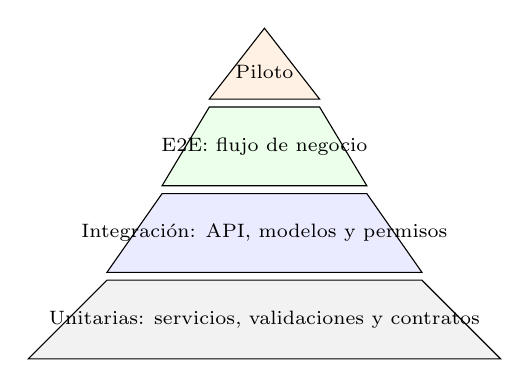
\begin{tikzpicture}[every node/.style={font=\scriptsize}]
\draw[fill=gray!10] (0,0) -- (6,0) -- (5,1) -- (1,1) -- cycle; \node at (3,0.5) {Unitarias: servicios, validaciones y contratos};
\draw[fill=blue!8] (1,1.1) -- (5,1.1) -- (4.3,2.1) -- (1.7,2.1) -- cycle; \node at (3,1.6) {Integración: API, modelos y permisos};
\draw[fill=green!8] (1.7,2.2) -- (4.3,2.2) -- (3.7,3.2) -- (2.3,3.2) -- cycle; \node at (3,2.7) {E2E: flujo de negocio};
\draw[fill=orange!10] (2.3,3.3) -- (3.7,3.3) -- (3,4.2) -- cycle; \node at (3,3.65) {Piloto};
\end{tikzpicture}
%
}
\caption{Pirámide de pruebas: distribución de la estrategia de cobertura por capas. Fuente: Elaboración propia.}
\label{fig:piramide-pruebas-integrada}
\end{figure}

\section{Trazabilidad de la validación: de los objetivos a las pruebas}
\label{sec:trazabilidad-validacion}

Para verificar que la validación del sistema cubriera todos los objetivos del proyecto, se estableció una matriz de trazabilidad que relaciona cada objetivo específico con las pruebas diseñadas para evaluarlo. Esta matriz, presentada en la Tabla \ref{tab:trazabilidad-pruebas}, permite a cualquier revisor académico comprobar qué afirmaciones de cumplimiento están respaldadas por evidencia de pruebas.

\begin{table}[!htbp]
\centering
\caption{Trazabilidad: objetivos del proyecto y pruebas de validación. Fuente: Elaboración propia.}
\label{tab:trazabilidad-pruebas}
\small
\def\TrzRow#1#2#3{\parbox[t]{3.0cm}{\raggedright #1} & \parbox[t]{9.0cm}{\raggedright #2} & \parbox[t]{2.5cm}{\raggedright #3}\\\hline}
\begin{tabular}{|l|l|l|}
\hline\ClassicTableHeader
\textbf{Objetivo específico} & \textbf{Pruebas de validación asociadas} & \textbf{Estado} \\
\hline
\TrzRow{1. Diagnosticar el flujo actual e identificar fallas críticas}{Inventario documental, flujo de 14 pasos documentado y cinco fallas críticas sustentadas en documentos de la empresa.}{Cumplido en diagnóstico documental}
\TrzRow{2. Diseñar la arquitectura funcional y técnica}{Arquitectura, modelo de datos, decisiones de diseño y matriz RBAC documentadas.}{Cumplido en diseño}
\TrzRow{3. Implementar los módulos principales}{Suite automatizada documentada para autenticación, RBAC, reglas de negocio, generación PDF, evidencias y módulos de seguimiento.}{Cumplido con evidencia técnica}
\TrzRow{4. Validar el funcionamiento del sistema}{Pruebas técnicas ejecutadas, escenarios de validación por rol definidos y lineamientos para piloto operativo.}{Parcial: piloto operativo pendiente}
\hline
\end{tabular}
\end{table}

\section{Recomendaciones para la validación en entorno productivo}
\label{sec:recomendaciones-validacion}

La validación realizada en el entorno de desarrollo constituye una base sólida, pero no sustituye la validación en un entorno productivo con usuarios reales y datos operativos auténticos. A continuación se proponen lineamientos para la fase de validación productiva que CERMONT S.A.S. debería ejecutar como siguiente paso:

\begin{enumerate}
    \item \textbf{Prueba piloto controlada:} Seleccionar un conjunto representativo de órdenes de trabajo reales que cubra los principales tipos de servicio y ejecutarlas completamente a través del sistema, desde la solicitud hasta el cierre administrativo, documentando tiempos, incidencias y observaciones de los usuarios.
    \item \textbf{Medición de línea base y post-implementación:} Establecer mediciones de los indicadores definidos en la metodología (tiempo de planeación, completitud documental, trazabilidad de evidencias) antes y después de la adopción del sistema, utilizando los mismos criterios de medición en ambos momentos para permitir comparaciones válidas.
    \item \textbf{Encuesta de satisfacción de usuarios:} Aplicar un instrumento estandarizado como el System Usability Scale (SUS) a los usuarios del sistema después de un periodo de uso suficiente, segmentando los resultados por rol para identificar diferencias en la experiencia de uso entre perfiles.
    \item \textbf{Auditoría de seguridad independiente:} Complementar la revisión OWASP Top 10 realizada durante el desarrollo con una auditoría de seguridad externa que evalúe la infraestructura de despliegue, la configuración del servidor y la protección de datos en el entorno productivo.
\end{enumerate}

Estas recomendaciones no constituyen resultados del proyecto, sino orientaciones para la continuidad del trabajo durante y después de la práctica empresarial. Su ejecución permitiría transformar los indicadores actualmente marcados como ``pendiente por medir'' en resultados cuantitativos verificables.

\section{Estrategia ampliada de pruebas por capas}
\label{sec:estrategia-ampliada-pruebas-capas}

La validación del aplicativo debe organizarse por capas para evitar confundir compilación, pruebas unitarias, pruebas funcionales y validación operativa. Que el sistema compile no significa que resuelva el proceso de negocio; que una prueba unitaria pase no significa que el usuario pueda cerrar una orden; y que una pantalla funcione no significa que la empresa haya reducido tiempos. Por ello, se propone una estrategia escalonada.

\begin{table}[!htbp]
\centering
\footnotesize
\caption{Estrategia de pruebas por capa del aplicativo. Fuente: elaboración propia.}
\label{tab:estrategia-pruebas-capas-ampliada}
\begin{adjustbox}{max width=\textwidth}
\begin{tabular}{|p{2.8cm}|p{4.4cm}|p{4.4cm}|p{3.2cm}|}
\hline\ClassicTableHeader
\textbf{Capa} & \textbf{Qué verifica} & \textbf{Evidencia esperada} & \textbf{Riesgo mitigado}\\
\hline
Typecheck & Compatibilidad de tipos y contratos. & Salida de comando sin errores. & Payloads inconsistentes.\\
Lint & Estilo, reglas de código y errores comunes. & Reporte de lint. & Deuda técnica temprana.\\
Unitarias & Servicios, validaciones y reglas de negocio aisladas. & Resultados de Vitest u otra herramienta. & Reglas rotas en módulos críticos.\\
Integración & Comunicación entre ruta, servicio, modelo y contrato. & Pruebas API o escenarios controlados. & Endpoints desconectados.\\
Frontend & Estados de carga, vacío, error y ready. & Capturas, pruebas de interfaz o revisión funcional. & Pantallas sin datos o con rutas rotas.\\
E2E & Flujo completo desde solicitud hasta cierre parcial. & Escenario documentado con pasos y resultado. & Módulos que funcionan aislados pero no integrados.\\
Operativa & Uso real con usuarios y órdenes. & Actas, mediciones y observaciones. & Afirmaciones de impacto no verificadas.\\
\hline
\end{tabular}
\end{adjustbox}
\end{table}

\section{Escenarios de validación funcional derivados del flujo de 14 pasos}
\label{sec:escenarios-validacion-funcional}

Los escenarios de validación deben derivarse de las fallas reales. Un escenario mínimo para planeación debe comprobar que una orden no avance a ejecución si el paquete de recursos está incompleto. Un escenario de evidencias debe comprobar que una foto o soporte quede asociado a la orden correcta. Un escenario de informes debe comprobar que el documento se genere usando datos capturados y no información escrita manualmente desde cero. Un escenario de cierre debe comprobar que SES, factura y pago se relacionen con la misma orden. Un escenario de costos debe comprobar que una línea de costo real pueda vincularse a una propuesta o actividad.

\begin{longtable}{|p{3.0cm}|p{4.6cm}|p{4.5cm}|p{2.6cm}|}
\caption{Escenarios de validación funcional propuestos. Fuente: elaboración propia.}
\label{tab:escenarios-validacion-funcional}\\
\hline\ClassicTableHeader
\textbf{Escenario} & \textbf{Pasos de usuario} & \textbf{Resultado esperado} & \textbf{Estado}\\
\hline
\endfirsthead
\hline\ClassicTableHeader
\textbf{Escenario} & \textbf{Pasos de usuario} & \textbf{Resultado esperado} & \textbf{Estado}\\
\hline
\endhead
\hline
\multicolumn{4}{r}{Continúa en la siguiente página}\\
\endfoot
\hline
\endlastfoot
Planeación completa & Crear orden, agregar recursos, verificar herramientas, cargar documentos HES y aprobar planeación. & La orden queda lista para ejecución sin bloqueadores críticos. & Pendiente de evidenciar con captura o prueba.\\
Ejecución con evidencia & Iniciar ejecución, diligenciar checklist, anexar fotografías y cerrar sesión. & Las evidencias quedan vinculadas a la orden y disponibles para informe. & Según evidencia del repositorio.\\
Generación de informe & Seleccionar orden ejecutada, generar informe técnico y revisar PDF. & El documento contiene actividades, observaciones y soportes. & Parcial o implementado según código.\\
Cierre administrativo & Registrar acta, SES, factura y pago asociado a la orden. & La línea de tiempo muestra el estado administrativo completo. & Pendiente si no hay flujo E2E.\\
Control de costos & Registrar costos reales y compararlos contra propuesta. & El sistema muestra variación y soporte del costo. & Propuesto o parcial.\\
\end{longtable}

\section{Validación cualitativa con roles de usuario}
\label{sec:validacion-cualitativa-roles-ampliada}

La validación por roles permite comprobar que el sistema responda a necesidades de usuarios distintos. El técnico requiere registrar información en campo sin complejidad excesiva; el ingeniero residente necesita revisar planeación, evidencias e informes; el administrativo necesita saber qué documentos habilitan SES y facturación; la gerencia necesita consultar estado, bloqueadores y costos. Cada perfil evalúa un aspecto distinto de la utilidad del sistema.

Para evitar afirmaciones no verificadas, la validación cualitativa debe documentarse con instrumentos simples: checklist por rol, observaciones de uso, capturas de pantalla, errores detectados, tiempo aproximado de ejecución de tareas y comentarios. Si esos instrumentos aún no existen, el libro debe presentarlos como plan de validación y no como resultado.

\section{Criterios de aceptación para la fase piloto}
\label{sec:criterios-aceptacion-piloto}

Una fase piloto del sistema debería aceptarse si cumple condiciones mínimas: usuarios creados con roles correctos, órdenes registradas sin errores críticos, planeación asociada a cada actividad, evidencias vinculadas a la orden, informes generados sin recaptura completa, actas o soportes de cierre asociados, estados de SES y factura consultables, y ausencia de pérdida de información durante conectividad intermitente en los escenarios definidos. Estos criterios permiten que la empresa evalúe utilidad sin exigir inicialmente métricas financieras complejas.

La medición cuantitativa puede añadirse después de confirmar que el flujo operativo funciona. En ese momento se podrán comparar tiempos de preparación de informes, completitud documental y seguimiento de cierre antes y después del uso del aplicativo. Mientras esa medición no se realice, el resultado académico se limita a validación técnica y preparación metodológica del piloto.
